\subsection{Performance}

\autoref{figure:time-jit-interpreter} shows that the interpreter has far better performance than the JIT for short tests. As the test duration increases the JIT increases in performance, eventually stabilising at approximately 2x faster execution time than the interpreter.

\begin{figure}
    \centering
    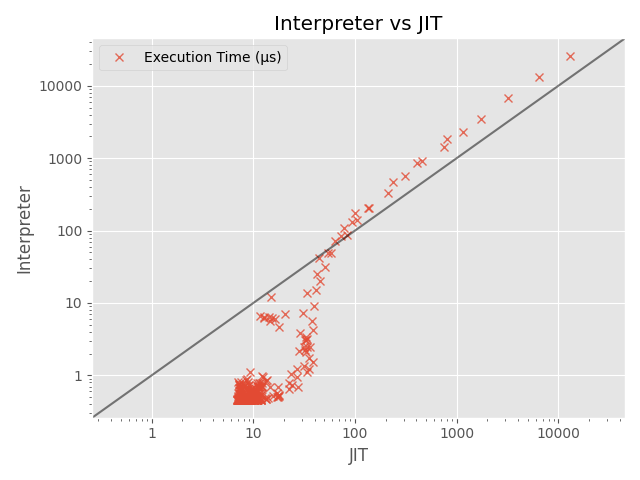
\includegraphics{output/graphs/scatter/time.png}
    \caption{Execution time of all tests for the JIT against the interpreter.}
    \label{figure:time-jit-interpreter}
\end{figure}

\subsubsection{Memory Intensive}

\subsubsection{Iteration}

\begin{figure}
    \centering
    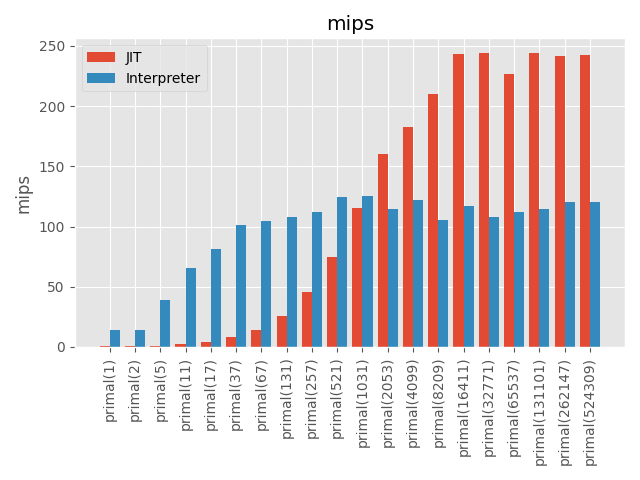
\includegraphics{output/graphs/tests/primal/mips.png}
    \caption{Performance in mips of the primal test suite.}
    \label{figure:primal-mips}
\end{figure}

\subsubsection{Recursion}

\begin{figure}
    \centering
    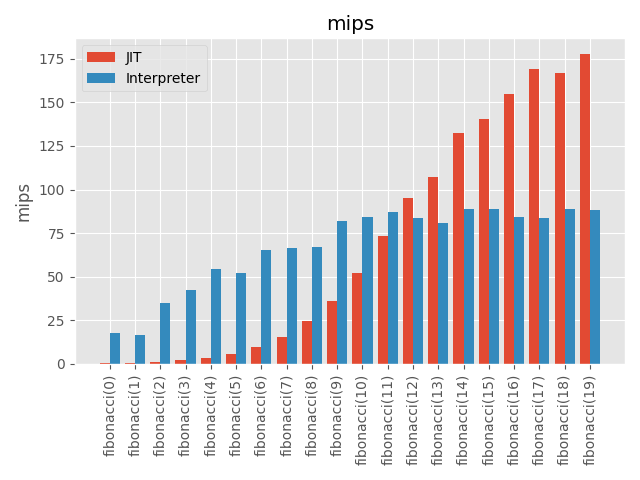
\includegraphics{output/graphs/tests/fibonacci/mips.png}
    \caption{Performance in mips of the fibonacci test suite.}
    \label{figure:fibonacci-mips}
\end{figure}